% Messwerte: Alle gemessenen Größen tabellarisch darstellen
% Auswertung: Berechnung geforderter Ergebnisse mit Schritten/Fehlerformeln/Erläuterung/Grafik (Programme)
\vfill

\section{Auswertung}
\label{sec:auswertung}

Zur graphischen Darstellung werden die Bibliotheken NumPy \cite{numpy} und Matplotlib \cite{matplotlib}
unter Python \cite{python} verwendet. Um nichtlineare Ausgleichsrechnungen mit einer Schätzung der
zugehörigen Abweichungen durchzuführen, kommt SciPy \cite{scipy} zum Einsatz. Speziell liefert die Funktion
\verb+scipy.optimize.curve_fit+ sowohl die optimalen Parameter, um die Fehlerquadrate zwischen Messdaten
und Modellverlauf zu minimieren, als auch die jeweilige Kovarianz $\sigma\raisebox{-0.2ex}{\(^2\)}$, aus der
direkt die Standardabweichung $\sigma$ bestimmt werden kann.

\newpage

\subsection{Gleichrichtungsverlauf und abgegriffene Intensität}

Unter Berücksichtigung von~\eqref{eqn:out} lässt sich eine phasenabhängige Modellfunktion
aufstellen, die im Folgenden zur nichtlinearen Regressionsrechnung dienen soll:
\begin{equation}
	U \hspace{-0.1ex} = a \cos(b \, \phi + c) + d
	\label{eqn:fit_1}
\end{equation}
\subsubsection{Rauschfreies Signal}
\begin{figure}
		\begin{subfigure}{0.3\textwidth}
		\centering
		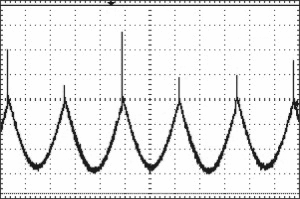
\includegraphics[height=3.21cm]{content/no_noise/0_no_noise.png}
		\caption{$\phi = \qty{0}{\degree}$}
	\end{subfigure}
	\hfill
	\begin{subfigure}{0.3\textwidth}
		\centering
		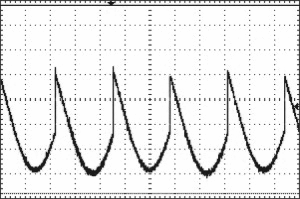
\includegraphics[height=3.21cm]{content/no_noise/30_no_noise.png}
		\caption{$\phi = \qty{30}{\degree}$}
	\end{subfigure}
	\hfill
	\begin{subfigure}{0.3\textwidth}
		\centering
		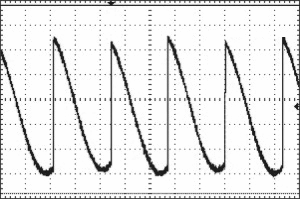
\includegraphics[height=3.21cm]{content/no_noise/60_no_noise.png}
		\caption{$\phi = \qty{60}{\degree}$}
	\end{subfigure}
	\par\bigskip
	\begin{subfigure}{0.3\textwidth}
		\centering
		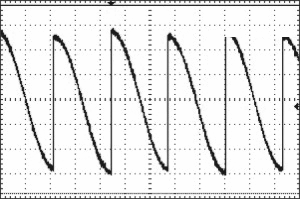
\includegraphics[height=3.21cm]{content/no_noise/90_no_noise.png}
		\caption{$\phi = \qty{90}{\degree}$}
	\end{subfigure}
	\hfill
	\begin{subfigure}{0.3\textwidth}
		\centering
		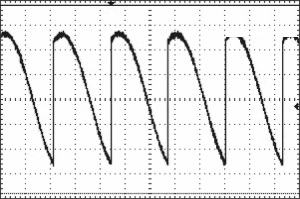
\includegraphics[height=3.21cm]{content/no_noise/120_no_noise.png}
		\caption{$\phi = \qty{120}{\degree}$}
	\end{subfigure}
	\hfill
	\begin{subfigure}{0.3\textwidth}
		\centering
		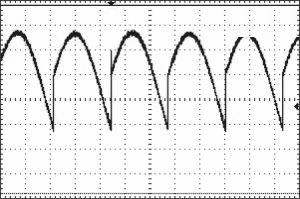
\includegraphics[height=3.21cm]{content/no_noise/150_no_noise.png}
		\caption{$\phi = \qty{150}{\degree}$}
	\end{subfigure}

	\captionsetup{width=0.975\linewidth}
	\caption{Spannungsverlauf $U_{\! \text{mix}}$ eines Sinussignals am Mischer für verschiedene Phasen.}
	\label{fig:mix_no_noise}
\end{figure}

Abbildung \ref{fig:mix_no_noise} zeigt die Verläufe des Mischsignals am Gleichrichter bei den angegebenen
Phasendifferenzen. Es ist zu erkennen, dass die Spannung dabei immer einer halben Periode des Ursprungssignals
folgt. Der jeweilige Abschnitt variiert mit der Verschiebung der Referenzspannung.

Aus den Werten in Tabelle \ref{tab:out_no_noise} ergeben sich für~\eqref{eqn:fit_1} die folgenden Parameter:
\begin{align*}
	&a = \input{build/a1.tex} &
	&b = \input{build/b1.tex} \\
	&d = \input{build/d1.tex} &
	&c = \input{build/c1.tex}
\end{align*}
Dabei entspricht $a$ der betragsmäßig maximalen Intensität. Die Variablen $b$, $c$ \mbox{und $d$}
charakterisieren entsprechende Verschiebungen und Stauchungen, die von der Erwartung
aus~\eqref{eqn:out} abweichen.

\begin{figure}[H]
	\includegraphics{build/plot_1a.pdf}
	\caption{Abgegriffene Gleichspannung $U_{\! \text{out}}$ zur Verschiebung $\phi$ mit passender
			 phasenabhängiger Ausgleichsrechnung.}
	\label{fig:out_no_noise}
\end{figure}
Die so parametrisierte Ausgleichskurve ist mit den Messaufzeichnungen aus Tabelle \ref{tab:out_no_noise}
in Abbildung \ref{fig:out_no_noise} dargestellt. Nach Betrachtung der Kenngrößen mit ihren Fehlern und
des graphischen Verlaufs entlang der Daten scheint die berechnete Funktion einen relativ hohen Deckungsgrad
zu erreichen.

\begin{table}[H]
	\vspace{1.35ex}
	\centering
	\captionsetup{width=0.75\linewidth}
	\caption{Messdaten der Ausgangsspannung $U_{\! \text{out}}$ zur relativen Phase.}
	\input{build/table_1a.tex}
	\label{tab:out_no_noise}
\end{table}

\subsubsection{Verrauschtes Signal}

\begin{figure}
		\begin{subfigure}{0.3\textwidth}
		\centering
		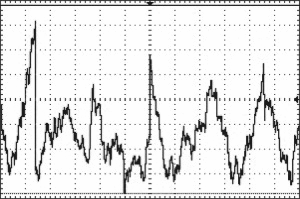
\includegraphics[height=3.21cm]{content/with_noise/0_with_noise.png}
		\caption{$\phi = \qty{0}{\degree}$}
	\end{subfigure}
	\hfill
	\begin{subfigure}{0.3\textwidth}
		\centering
		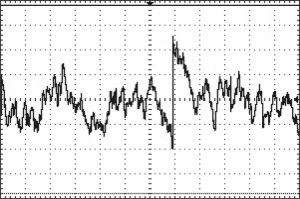
\includegraphics[height=3.21cm]{content/with_noise/30_with_noise.png}
		\caption{$\phi = \qty{30}{\degree}$}
	\end{subfigure}
	\hfill
	\begin{subfigure}{0.3\textwidth}
		\centering
		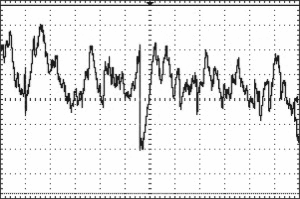
\includegraphics[height=3.21cm]{content/with_noise/60_with_noise.png}
		\caption{$\phi = \qty{60}{\degree}$}
	\end{subfigure}
	\par\bigskip
	\begin{subfigure}{0.3\textwidth}
		\centering
		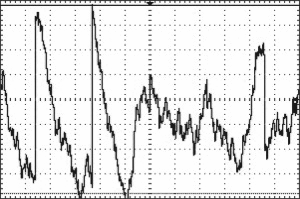
\includegraphics[height=3.21cm]{content/with_noise/90_with_noise.png}
		\caption{$\phi = \qty{90}{\degree}$}
	\end{subfigure}
	\hfill
	\begin{subfigure}{0.3\textwidth}
		\centering
		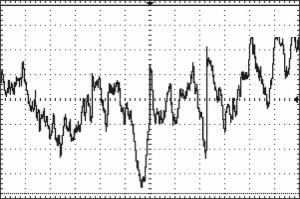
\includegraphics[height=3.21cm]{content/with_noise/120_with_noise.png}
		\caption{$\phi = \qty{120}{\degree}$}
	\end{subfigure}
	\hfill
	\begin{subfigure}{0.3\textwidth}
		\centering
		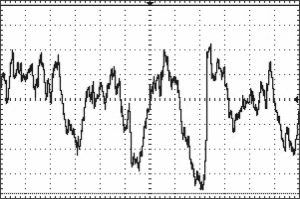
\includegraphics[height=3.21cm]{content/with_noise/150_with_noise.png}
		\caption{$\phi = \qty{150}{\degree}$}
	\end{subfigure}

	\captionsetup{width=0.975\linewidth}
	\caption{Spannungsverlauf $U_{\! \text{mix}}$ eines Sinussignals am Mischer für verschiedene Phasen.}
	\label{fig:mix_with_noise}
\end{figure}

Verglichen mit Abbildung \ref{fig:mix_no_noise} lassen sich aus den Verläufen der verrauschten Mischsignale
in Abbildung \ref{fig:mix_with_noise} kaum mehr Informationen über die Messgröße ablesen. Stark eingeschränkt
kann anhand der Peaks noch die Frequenz der Referenzspannung $U_{\! \text{ref}}$ erkannt werden. 

\begin{table}[H]
	\vspace{1.35ex}
	\centering
	\captionsetup{width=0.75\linewidth}
	\caption{Messdaten der Ausgangsspannung $U_{\! \text{out}}$ zur relativen Phase.}
	\input{build/table_1b.tex}
	\label{tab:out_with_noise}
\end{table}

Mit den Werten in Tabelle \ref{tab:out_with_noise} lässt sich die Regressionskurve zu den Daten in Abbildung
\ref{fig:out_with_noise} berechnen. Der Einfluss der einzelnen Merkmale entspricht der vorherigen Beschreibung.

\begin{figure}[H]
	\includegraphics{build/plot_1b.pdf}
	\caption{Abgegriffene Gleichspannung $U_{\! \text{out}}$ zur Verschiebung $\phi$ mit passender
			 phasenabhängiger Ausgleichsrechnung.}
	\label{fig:out_with_noise}
\end{figure}

Der Fit an~\eqref{eqn:fit_1} ist durch folgende Eigenschaften beschrieben:
\begin{align*}
	&a = \input{build/a2.tex} &
	&b = \input{build/b2.tex} \\
	&d = \input{build/d2.tex} &
	&c = \input{build/c2.tex}
\end{align*}
Trotz starker Rauschkomponente lässt sich also ein deutliches Signal messen, dessen Verlauf dem rauschfreien
Fall stark ähnelt. Die Streuung der Messungen um den Fit ist hier ebenfalls nicht signifikant stärker
ausgeprägt.

\newpage

\subsection{Abstandsabhängiger Intensitätsverlauf eines Lichtsignals}

Da sich die Leuchtdiode besonders für größere Entfernungen als Punktquelle nähern lässt, breitet sich ihre
Lichtintensität per Annahme gleichmäßig auf einer Kugeloberfläche aus. Damit kann das folgende mathematische
Modell genutzt werden:
\begin{equation}
	U = v \, r^{-2} + w
	\label{eqn:fit_2}
\end{equation}
\begin{figure}[H]
	\includegraphics{build/plot_2.pdf}
	\caption{Gemessene Intensität $U_{\! \text{out}}$ bei Abstand $r$ mit Ausgleichskurven.}
	\label{fig:photo-plot}
\end{figure}
Mit den Werten aus Tabelle \ref{tab:photo} lässt sich die nichtlineare Regression an~\eqref{eqn:fit_2}
durchführen. Die resultierenden Kurven sind in Abbildung \ref{fig:photo-plot} dargestellt. Um für die
Abweichung bei geringeren Abständen zu kompensieren, können die ersten drei Messungen ignoriert werden.
Dieses angepasste Vorgehen liefert $v = \input{build/r1.tex}$ als Koeffizienten, während die
Verschiebung $w$ ganz verschwindet. Dagegen ergeben sich für den regulären Ausgleich folgende Parameter:
\begin{align*}
	&v = \input{build/r2.tex} \\
	&w = \input{build/s2.tex}
\end{align*}
Das Signal der LED verschwindet nie vollständig am Photodetektor, da der Versuch durch die Länge der Schiene
begrenzt ist. Für den Maximalabstand lässt sich also mit $r_{\text{max}} > \qty{148}{\centi\meter}$ nur
eine untere Schranke festlegen.

\begin{table}[H]
	\centering
	\captionsetup{width=0.61\linewidth}
	\caption{Messdaten der auftretenden Spannung $U_{\! \text{out}}$ zum Abstand $r$ zwischen LED und PD.}
	\input{build/table_2.tex}
	\label{tab:photo}
	\vspace{1.23ex}
\end{table}
